%!TeX root=../tese.tex
\chapter{Álgebras de flag}
\label{cap:flag-algebras}


\newcommand{\rfsigma}{\mathbb{R}\mathcal{F}^\sigma}
\newcommand{\asigma}{\mathcal{A}^\sigma}

\newcommand{\emptyflag}{\varnothing}
\newcommand{\isom}{\cong}

% Tikz setup from https://arxiv.org/abs/2103.14179


\newcommand{\vc}[1]{\ensuremath{\vcenter{\hbox{#1}}}}
\tikzset{vtx/.style={inner sep=1.7pt, outer sep=0pt, circle, fill}}
\tikzset{unlabeled_vertex/.style={inner sep=1.7pt, outer sep=0pt, circle, fill, draw=black}}
\tikzset{labeled_vertex/.style={inner sep=2.2pt, outer sep=0pt, rectangle, fill=yellow, draw=black}}
\tikzset{edge_color0/.style={color=black,line width=1.2pt}}
\tikzset{edge_color1/.style={color=red,  line width=1.2pt,opacity=0}}
\tikzset{edge_color2/.style={color=blue, line width=1.2pt,opacity=1}}

\newcommand{\flagone}{ % this is the unlabeled triangle
  \vc{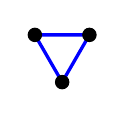
\begin{tikzpicture}[scale=0.5]
    \draw \foreach \x in {0,1,2}{(270+\x*360/3:0.8) coordinate(x\x)};
    \draw[edge_color2] (x0)--(x1)--(x2)--(x0);
    \draw (x0) node[unlabeled_vertex]{};
    \draw (x1) node[unlabeled_vertex]{};
    \draw (x2) node[unlabeled_vertex]{};
  \end{tikzpicture}}
}
\newcommand{\kthree}{\flagone}

\newcommand{\flagtwo}{ % this is the unlabeled edge
  \vc{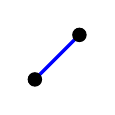
\begin{tikzpicture}[scale=0.5]
    \draw (225:0.8) coordinate(x0);
    \draw (45:0.8) coordinate(x1);
    \draw[edge_color2] (x0)--(x1);
    \draw (x0) node[unlabeled_vertex]{};
    \draw (x1) node[unlabeled_vertex]{};
  \end{tikzpicture}}
}
\newcommand{\edge}{\flagtwo}

\newcommand{\flagthree}{ % this represents the edges among non-neighbors of a vertex
  \vc{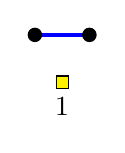
\begin{tikzpicture}[scale=0.5]
    \draw \foreach \x in {0,1,2}{(270+\x*360/3:0.8) coordinate(x\x)};
    \draw[edge_color2] (x1)--(x2);
    \draw (x0) node[labeled_vertex,label=below:$1$]{};
    \draw (x1) node[unlabeled_vertex]{};
    \draw (x2) node[unlabeled_vertex]{};
  \end{tikzpicture}}
}

\newcommand{\flagfour}{
  \vc{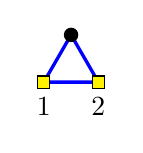
\begin{tikzpicture}[scale=0.5]
    \draw \foreach \x in {0,1,2}{(210+\x*360/3:0.8) coordinate(x\x)};
    \draw[edge_color2] (x0)--(x1)--(x2)--(x0);
    \draw (x0) node[labeled_vertex,label=below:$1$]{};
    \draw (x1) node[labeled_vertex,label=below:$2$]{};
    \draw (x2) node[unlabeled_vertex]{};
  \end{tikzpicture}}
}
\newcommand{\kthreeLabeledEdge}{\flagfour}

\newcommand{\flagfive}{ % this is the labeled edge
  \vc{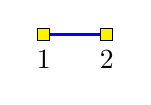
\begin{tikzpicture}[scale=0.5]
    \draw (180:0.8) coordinate(x0);
    \draw (360:0.8) coordinate(x1);
    \draw[edge_color2] (x0)--(x1);
    \draw (x0) node[labeled_vertex,label=below:$1$]{};
    \draw (x1) node[labeled_vertex,label=below:$2$]{};
  \end{tikzpicture}}
}
\newcommand{\labeledEdge}{\flagfive}

\newcommand{\flagsix}{ % this is the labeled non-edge
  \vc{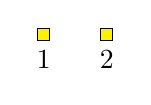
\begin{tikzpicture}[scale=0.5]
    \draw (180:0.8) coordinate(x0);
    \draw (360:0.8) coordinate(x1);
    \draw (x0) node[labeled_vertex,label=below:$1$]{};
    \draw (x1) node[labeled_vertex,label=below:$2$]{};
  \end{tikzpicture}}
}
\newcommand{\labeledNonEdge}{\flagsix}

\newcommand{\flagseven}{
  \vc{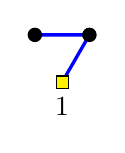
\begin{tikzpicture}[scale=0.5]
    \draw \foreach \x in {0,1,2}{(270+\x*360/3:0.8) coordinate(x\x)};
    \draw[edge_color2] (x0)--(x1)--(x2);
    \draw (x0) node[labeled_vertex,label=below:$1$]{};
    \draw (x1) node[unlabeled_vertex]{};
    \draw (x2) node[unlabeled_vertex]{};
  \end{tikzpicture}}
}

\newcommand{\flageight}{ % this is the labeled edge with an extra vertex joined to 1
  \vc{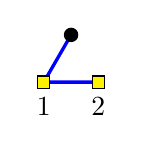
\begin{tikzpicture}[scale=0.5]
    \draw \foreach \x in {0,1,2}{(210+\x*360/3:0.8) coordinate(x\x)};
    \draw[edge_color2] (x2)--(x0)--(x1);
    \draw (x0) node[labeled_vertex,label=below:$1$]{};
    \draw (x1) node[labeled_vertex,label=below:$2$]{};
    \draw (x2) node[unlabeled_vertex]{};
  \end{tikzpicture}}
}

\newcommand{\flagnine}{ % this is the labeled edge with an extra vertex joined to 2
  \vc{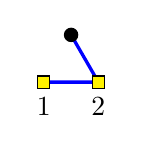
\begin{tikzpicture}[scale=0.5]
    \draw \foreach \x in {0,1,2}{(210+\x*360/3:0.8) coordinate(x\x)};
    \draw[edge_color2] (x0)--(x1)--(x2);
    \draw (x0) node[labeled_vertex,label=below:$1$]{};
    \draw (x1) node[labeled_vertex,label=below:$2$]{};
    \draw (x2) node[unlabeled_vertex]{};
  \end{tikzpicture}}
}

\newcommand{\flagten}{
  \vc{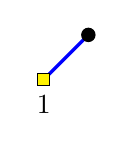
\begin{tikzpicture}[scale=0.5]
    \draw (225:0.8) coordinate(x0);
    \draw (45:0.8) coordinate(x1);
    \draw[edge_color2] (x0)--(x1);
    \draw (x0) node[labeled_vertex,label=below:$1$]{};
    \draw (x1) node[unlabeled_vertex]{};
  \end{tikzpicture}}
}
\newcommand{\edgeWithOneLabel}{\flagten}

\newcommand{\flageleven}{
  \vc{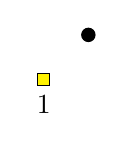
\begin{tikzpicture}[scale=0.5]
    \draw (225:0.8) coordinate(x0);
    \draw (45:0.8) coordinate(x1);
    \draw (x0) node[labeled_vertex,label=below:$1$]{};
    \draw (x1) node[unlabeled_vertex]{};
  \end{tikzpicture}}
}
\newcommand{\nonEdgeWithOneLabel}{\flageleven}

\newcommand{\flagtwelve}{
  \vc{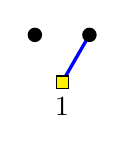
\begin{tikzpicture}[scale=0.5]
    \draw \foreach \x in {0,1,2}{(270+\x*360/3:0.8) coordinate(x\x)};
    \draw[edge_color2] (x0)--(x1);
    \draw (x0) node[labeled_vertex,label=below:$1$]{};
    \draw (x1) node[unlabeled_vertex]{};
    \draw (x2) node[unlabeled_vertex]{};
  \end{tikzpicture}}
}

A estrutura desse capítulo segue fortemente o que é apresentado em~\cite{marcel2016flag} e também inspirado nas lecture notes do Andrzej Grzesik.

\section{Preliminares}

Seja $k \geq 0$ um inteiro.
Um \emph{tipo} de \emph{tamanho} $k$ é um grafo $G$ com $V(G) = [k]$,
i.e. é um grafo com todos os seus vértices rotulados com os inteiros de $1$ a $k$.
O tipo vazio (grafo vazio) é denotado por $\emptyflag$.

Seja $\sigma$ um tipo de tamanho $k$ e $F$ um grafo com pelo menos $k$ vértices.
Um \emph{$\sigma$-flag} é um par $(F,\theta)$ em que $\theta \colon [k] \to V(F)$
é um homomorfismo de grafos injetor tal que $F[\theta([k])] \isom \sigma$.
Em outras palavras, $\sigma$-flag é um grafo \emph{parcialmente} rotulado, em que o subgrafo rotulado é uma cópia de $\sigma$.

Note que todo tipo $\sigma$ é um $(\sigma,\theta)$-flag para $\theta$ a função identidade em $[k]$.
Em geral, iremos omitir $\theta$ da definição de um flag se a sua definição for clara do contexto.

Para definir isomorfismos entre $\sigma$-flags, fazemos exatamente como para grafos, com a condição adicional que os rótulo devem ser preservados pela bijeção.
Formalmente, dizemos que dois $\sigma$-flags $(G_1,\theta_1)$ e $(G_2,\theta_2)$ são \emph{isomórficos} se existe um isomorfismo $\theta \colon V(G_1) \to V(G_2)$ tal que $\theta(\theta_1(i))=\theta_2(i)$ para cada $i \in [|\sigma|]$.

\begin{example}

\begin{enumerate}
  \item Sejam \[\sigma_1=\labeledEdge \qquad \text{e} \qquad \sigma_2=\labeledNonEdge \]
  dois tipos (ambos com $k=2$ vértices).
  Então se $G=\kthreeLabeledEdge$ e $\theta$ é a identidade em $\{1,2\}$, temos que $(G,\theta)$ é um $\sigma_1$-flag mas não é um $\sigma_2$-flag.

  Usando a notação apresentada anteriormente, podemos simplesmente escrever que $G$ é um $\sigma_1$-flag.
  
  \item $\kthree$ é um $\emptyflag$-flag, uma vez que nenhum de seus vértices está rotulado.
  
  \item $\flagthree$ é um $\sigma_3$-flag, onde $\sigma_3$ é o (único) tipo com exatamente um vértice.
  $\flagseven$ é outro $\sigma_3$-flag.
  
  \item $\flageight$ e $\flagnine$ são dois $\labeledEdge$-flags, que são isomórficos como grafos mas não são isomórficos como flags.
\end{enumerate}

\end{example}

Finalmente, para cada tipo $\sigma$ e $n \geq |\sigma|$, definimos $\mathcal F_n^\sigma$ como o conjunto de todos os $\sigma$-flags de tamanho $n$.

\subsection{Densidade e limites}

Para continuar a definição de flag algebras, será importante definir densidades e suas propriedas.
Sejam $F$ e $G$ dois grafos (sem rótulos especiais nos vértices) e defina $c(F,G)$ como a quantidade de subgrafos \emph{induzidos} de $G$ que são isomorfos a $f$.
Então definimos a \emph{densidade de $F$ em $G$} como \[ p(F,G) \coloneqq \frac{c(F,G)}{\binom{|G|}{|F|}}. \]
De outra forma, $p(F;G) = \prob_U [G[U] \isom F]$ é a probabilidade que um subconjunto $U$ de $V(G)$ com tamanho exatamente $|F|$ induza um subgrafo isomorfo a $F$.

Por exemplo, temos $p(K_2;G) = \frac{e(G)}{\binom{n}{2}}$ e $p(K_3;G)$ é a probabilidade de uma tripla de vértices distintos de $G$ escolhida uniformemente ao acaso formar um triângulo.

De forma similar, para um tipo $\sigma$ dado, um $\sigma$-flag $(G,\theta)$ e um conjunto de $\sigma$-flags $F_1,F_2,\dots,F_t$, deifnimos a \emph{densidade de $F_1,F_2,\dots,F_t$ em $G$} como a probabilidade que conjuntos $U_1,U_2,\dots,U_t \subseteq V(G) \setminus \text{Im } \theta$ dois a dois disjuntos escolhidos uniformemente ao acaso satisfaçam $(G[U_i \cup \text{Im } \theta], \theta) \isom F_i$ para cada $i \in \{1,2,\dots,t\}$.
Denotamos essa densidade como $p(F_1,F_2,\dots,F_t;G)$.

\begin{example}
  Seja $\sigma$ o tipo de tamanho $1$.
  Sejam $F_1=\edgeWithOneLabel, F_2=\nonEdgeWithOneLabel, G=\flagseven$ três $\sigma$-flags.
  Então $p(F_1,F_2;G) = \frac12$.
\end{example}

Os dois seguintes lemas fornecem as relações para a ``regra da cadeia'' das densidades.

\begin{lemma}\label{lem:chain-rule-2}
  Sejam $F$ e $G$ dois $\sigma$-flags.
  Se $n$ é um inteiro positivo tal que $|F| \leq n \leq |G|$, então
  \[
    p(F;G) = \sum_{F' \in \mathcal F_n^\sigma} p(F;F')p(F';G).
  \]
\end{lemma}

\begin{lemma}\label{lem:chain-rule-many}
  Suponha que $F_1,F_2,\dots,F_t$ e $G$ são $\sigma$-flags.
  Se $n$ é um inteiro positivo tal que 
  \[
    \sum_{i=1}^t (|F_i|-|\sigma|) \leq n-|\sigma| \leq |G|-|\sigma|,
  \]
  então para todo $s \in [t]$ vale
  \[
    p(F_1,F_2,\dots,F_t;G) = \sum_{F \in \mathcal F_n^\sigma} p(F_1,F_2,\dots,F_s;F)p(F,F_{s+1},F_{s+2}\dots,F_t;G)
  \]
\end{lemma}

Agora, podemos definir a noção de funcionais limites e álgebras de flag.

\begin{definition}
  Uma sequência de grafos $(G_1,G_2,\dots)$ é chamada de \emph{crescente} se $(|G_1|,|G_2|,\dots)$ é estritamente crescente.
  Uma sequência crescente de grafos é chamada de \emph{convergente} se para todo grafo $F$ vale que a sequência
  \[ (p(F;G_1),p(F;G_2),\dots) \]
  é convergente.
\end{definition}

\begin{example}

\begin{enumerate}
  \item A sequência de grafos completos $(K_1,K_2,K_3,\dots)$ é convergente.
  \item A sequência de grafos bipartidos completos em que uma classe tem o tamanho da outra também é convergente: $(K_{1,2},K_{2,4},K_{3,6},\dots)$.
  \item A sequência de grafos de Andrásfai $(F_1,F_2,F_3,\dots)$ (que serão estudados no Capítulo~\ref{cap:grau-limitado}) é um exemplo menos trivial de sequência convergente.
  \item Se $G$ é um grafo qualquer.
  Então a sequência $(G_k)_{k \geq 0}$, onde $G_0=G$ e $G_k$ é um blow-up de $G$ em que cada vértice é substituído por um conjunto independente de tamanho $k+1$ é convergente.
  \item Pelo Teorema de Tychonoff (ADICIONAR REFERÊNCIA), toda sequẽncia crescente de grafos possui uma subsequência decrescente.
\end{enumerate}

\end{example}

Sequências convergentes e crescentes de $\sigma$-flags são definidas de forma análoga para qualquer tipo $\sigma$.
Para cada sequência convergente de $\sigma$-flags $(A_1,A_2,\dots)$, podemos definir uma função $\phi$ que atribui a cada $\sigma$-flag $F$ o real $\phi(F) \coloneqq \lim_{k \to \infty} p(F;A_k)$.
A tais funções $\phi$ chamamos de \emph{limites funcionais}.

Na seção~\ref{sec:estrutura-algebrica}, iremos apresentar uma estrutura algébrica para flags the permitirão desenvolver propriedades gerais de limites funcionais.
Então, na seção~\ref{sec:aplicacoes}, mostraremos como traduzir os resultados obtidos para limites funcionais para a linguagem clássica de grafos e aplicá-las ao nosso problema.

\subsection{Estrutura algébrica}\label{sec:estrutura-algebrica}

Agora, vamos colocar uma estrutura algébrica para os flags.

Seja $\rfsigma$ o espaço vetorial gerado pelas combinações lineares de $\sigma$-flags com coeficientes (isto é, o espaço de somas formais de múltiplos reais de $\sigma$-flags).
Podemos estender linearmente qualquer limite funcional para $\rfsigma$.

Utilizando o Lema~\ref{lem:chain-rule-2}, obtém-se que para qualquer $\sigma$-flag $F$ e $n \geq |F|$ vale
\[ \phi(F) = \phi\left( \sum_{F' \in \mathcal F_n^\sigma} p(F;F')F' \right), \]
ou seja,
\begin{equation}\label{eq:guys-in-kernel}
  F - \sum_{F' \in \mathcal F_n^\sigma} p(F;F')F' \in \ker\phi
\end{equation}
para todo funcional limite $\phi$.
Podemos então definir o espaço vetorial $\asigma \coloneqq \rfsigma / \mathcal K^\sigma$, sendo $\mathcal K^\sigma$ o subespaço gerado por todos os vetores na forma~\ref{eq:guys-in-kernel}.
Note que $\phi(\sigma) = p(\sigma;F) = 1$ para todo $\sigma$-flag $F$, logo $\asigma$ tem pelo menos um elemento não nulo.

A principal vantagem de trabalhar com $\asigma$ é que é possível definir multiplicação entre seus elementos (transformando esse espaço vetorial em uma álgebra de fato).

\begin{definition}
  Sejam $F$ e $G$ $\sigma$-flags e seja $n \geq |F|+|G|-|\sigma|$.
  Definimos o produto de $F$ e $G$ como
  \[ F \cdot G = \left( \sum_{H \in \mathcal F_n^\sigma} p(F,G;H)H \right) + \mathcal K^\sigma \in \asigma. \]
\end{definition}

É possível provar que o produto acima está bem definido, é comutativo e associativo.

\begin{example}
  Sejam $F_1 = \edgeWithOneLabel$ e $F_2 = \nonEdgeWithOneLabel$. Então $F \cdot G = \frac12 \flagseven + \frac12 \flagtwelve$.
\end{example}

Agora, podemos enunciar o principal resultado das álgebras de flag.

\begin{theorem}[$\phi$ é homomorfismo de $\asigma$ para $\mathbb R)$]
  Se $f,g$ são dois elementos da álgebra $\asigma$ e $\phi$ é um funcional limite qualquer, então
  \[ \phi(f \cdot g) = \phi(f) \cdot \phi(g). \]
\end{theorem}

\subsection{Operador de média}

Em teoria extremal de grafos, estamos interessados em obter resultados sobre a densidade de grafos (pequenos) \textit{não rotulados} em grafos maiores.
Então por que usamos flags, isto é, grafos rotulados?
Mesmo para teoremas simples (como o Teorema~\ref{thm:mantel-com-flag}), costuma ser muito difícil obter resultados úteis usando apenas a álgebra $\aempty$.

A estratégia geral será produzir relação válidas em uma álgebra $\asigma$ e então aplicar uma transformação linear de $\asigma$ para $\aempty$ que chamaremos de \emph{operador de média}.

\begin{definition}
  Seja $F$ um $\sigma$-flag, onde $\sigma$ é um tipo de tamanho $k$.
  Definimos $\downarrow F$ como o $\emptyflag$-flag obtido ao esquecer os rótulos dados aos vértices de $F$.
  Definimos também $q(F)$ como a probabilidade de que uma função injetiva $\theta \colon [k] \to V(F)$ escolhida uniformemente ao acaso é tal que $(\downward F,\theta) \isom F$.

  Então definimos $\average{F}=q(F) \downward F$, e estendemos $\average\cdot$ linearmente para $\mathbb R \mathcal{F}^\sigma$ para obter uma transformação linear de $\mathbb R \mathcal{F}^\sigma$ para $\mathbb R \mathcal{F}^\emptyflag$.
\end{definition}

O seguinte teorema, junto com o Lema~\ref{lem:chain-rule-2}, prova the $\average{K^\sigma} \subseteq \mathcal K^\emptyflag$, e portanto $\average\cdot$ também é uma transformação bem definida de $\asigma$ para $\aempty$.

\begin{theorem}\label{thm:expected-average-embedding}
  Sejam $F$ um $\sigma$-flag e $G$ um $\emptyflag$-flag com $|G| \geq |F|$ e $p(\downward\sigma;G)>0$.
  Se $\theta$ é um embedding de $\sigma$ em $G$ escolhido uniformemente ao acaso, então
  \[ \mathbb E[p(F;(G,\theta))] = \frac{q(F)p(\downward F;G)}{q(\sigma)p(\downward \sigma;G)}. \]
\end{theorem}

De fato, o que o Teorema~\ref{thm:expected-average-embedding} diz é que o operador de média $\average{\cdot}$ atua da seguinte forma:
para cada subgrafo induzido de $G$ isomorfo a $\sigma$, se calcula a densidade de $F$ em $G$ ao se considerar $G$ como um $\sigma$-flag rotulado dessa mesma forma e se calcula o valor esperado dessa densidade.

Considere por exemplo o flag $\edgeWithOneLabel$.
Então $\average{\edgeWithOneLabel}=\edge$ e
\[ \mathbb E\left[p\left(\edge;(G,\theta)\right)\right] = p(E;G), \]
ou seja, o valor esperado da proporção de vizinhos de um vértice escolhido ao acaso é (assintoticamente) igual à densidade de arestas no grafo.

A mesma ideia pode ser aplicada para combinações de flags mais sofisticadas:
o operador de média aplicado ao flag $\left(\edgeWithOneLabel - \nonEdgeWithOneLabel\right)^2$
calcula (assintoticamente) a variância da diferença da proporção entre vizinhos e não vizinhos de vértices em um grafo e.
Além disso, a linearidade do operador permite avaliar esse indicador que (a princípio) é quadrático em função de combinações lineares de $\emptyflag$-flags.
A prova do Teorema de Mantel na Seção~\ref{sec:mantel-com-flag} mostrará o poder dessa ideia.

\subsection{Teorema de Mantel}~\label{sec:mantel-com-flag}
Começamos com o clássico Teorema de Mantel.
Mostraremos como expressar o Teorema usando a linguagem de álgebras de flag bem como recuperá-lo dos resultados com álgebras de flag.

\begin{theorem}[``Mantel'']~\label{thm:mantel-com-flag}
  Seja $\phi$ um funcional limite qualquer.
  Se $\phi\left(\kthree\right) = 0$, então $\phi\left(\edge\right) \leq \frac12$.
\end{theorem}

Em alto nível, o Teorema~\ref{thm:mantel-com-flag} pode ser visto como uma versão assintótica do Teorema~\ref{thm:mantel}: para grafos grandes, se a proporção de vértices que são triângulos tende a $0$, então a proporção de áreas tende a no máximo $1/2$.

Antes de provar o Teorema~\ref{thm:mantel-com-flag}, vamos ver como obter o Teorema~\ref{thm:mantel} do Teorema~\ref{thm:mantel-com-flag}.
Para definir um funcional limite $\phi$, precisamos de uma sequência convergente de grafos.
Toda sequência crescente de grafos possui uma subsequência convergente.
Assim, seja $(G_k)_{k \geq 0}$ uma sequência convergente de grafos livres de triângulos em que $G_{i+1}$ é um blow-up de $G_i$ para cada $i \geq 0$ e $G_0$ é o grafo para que se quer provar o Teorema~\ref{thm:mantel}.
O Teorema~\ref{thm:mantel-com-flag} pode ser escrito como $e(G_k) \leq (\frac14+o_k(1))|G_k|^2$, onde $o_k(1)$ é uma função que tende a zereo quando $k$ cresce.

Mas pela definição da sequência $G_k$, temos
\[e(G_k)=\frac{|G_k|^2}{|G_0|^2}e(G_0) \leq (\frac14+o_k(1))|G_k|^2.\]
Logo, $e(G_0)/|G_0|^2 \leq (1/4+o_k(1))$, e segue que $e(G_0)/|G_0|^2 \leq 1/4$, como desejado.

A prova a seguir reflete a estratégia geral que será utilizada para provas com álgebras de flag.

\begin{proof}[Prova do Teorema~\ref{thm:mantel-com-flag}]
  Seja $\sigma$ o tipo de tamanho $1$ e considere o vetor \[v=\edgeWithOneLabel-\nonEdgeWithOneLabel \in \asigma.\]
  Veja que para qualquer homomorfismo $\psi \colon \asigma \to \mathbb R$ temos $\psi(v^2) = \psi(v)^2 \geq 0$.
  Observe também que
  \begin{align*}
    v^2 &= \left(\edgeWithOneLabel-\nonEdgeWithOneLabel\right)^2 \\
        &= \edgeWithOneLabel^2 - 2\edgeWithOneLabel\cdot\nonEdgeWithOneLabel + \nonEdgeWithOneLabel^2 \\
        &= \left(\cherry + \kthreeLabeledVertex\right) - 2\left(\frac12 \flagseven + \frac12 \flagtwelve\right) + \left(\flagthree + \flagfifteen\right),
  \end{align*}

  logo tomando $\psi = \phi \circ \average\cdot$, obtemos

  \begin{align}
    \psi(v^2) &= \phi\left(\average{\cherry}+\average{\kthreeLabeledVertex}-\average{\flagseven}-\average{\flagtwelve}+\average{\flagthree}+\average{\flagfifteen}\right) \nonumber \\
    &= \frac13\phi\left(\unlabeledCherry\right) + \phi\left(\kthree\right) - \frac23\phi\left(\unlabeledCherry\right)-\frac23\phi\left(\unlabeledCherryComplement\right)+\frac13\phi\left(\unlabeledCherryComplement\right)+\phi\left(\flageighteen\right) \nonumber \\
    &=\phi\left(\kthree - \frac13 \unlabeledCherry - \frac13 \unlabeledCherryComplement{} + \flageighteen\right) \geq 0.\label{eq:phi-relation-1}
  \end{align}

  Assim, obtemos uma relação (não trivial) sobre funcionais limites com relação a $\emptyflag$-flags de tamanho $3$.
  Porém, o resultado do Teorema diz respeito a $\edge$, que é um $\emptyflag$ de tamanho $2$.
  Para associar os dois, usamos a expressão de~\ref{eq:guys-in-kernel}, que é igual a zero em $\aempty$.
  Tomando $F=\kthree, n=2$, obtemos
  \begin{equation}\label{eq:3-to-1}
    \justavertex = \kthree + \unlabeledCherry + \unlabeledCherryComplement{} + \flageighteen.
  \end{equation}
  De forma similar, para $F=\kthree, n=3$, obtemos
  \begin{equation}\label{eq:3-to-2}
    \edge = \kthree + \frac23 \unlabeledCherry + \frac13 \unlabeledCherryComplement.
  \end{equation}
  Combinando~\ref{eq:3-to-2} e~\ref{eq:phi-relation-1}:
  \begin{align}
    \phi\left(\edge\right) &\leq \phi\left(\kthree + \frac23 \unlabeledCherry + \frac13 \unlabeledCherryComplement\right) + \frac12\phi\left(\kthree - \frac13 \unlabeledCherry - \frac13 \unlabeledCherryComplement + \flageighteen\right) \nonumber \\
    &= \frac12\phi\left(\kthree + \unlabeledCherry + \unlabeledCherryComplement + \flageighteen\right) + \phi\left(\kthree\right) - \frac13\phi\left(\unlabeledCherryComplement\right) \nonumber \\
    &\leq \frac12\phi\left(\justavertex\right) + \phi\left(\kthree\right) \label{eq:phi-relation-2} \\
    &= \frac12 \nonumber,
  \end{align}
  onde na última igualdade usamos que $\phi\left(\justavertex\right)=1$ para todo funcional limite $\phi$ e também a condição que $\phi\left(\kthree\right)=0$.
\end{proof}

A prova acima do Teorema de Mantel, ainda que aparentemente complicada, serve de exemplo de diversas propriedades e vantagens do método de álgebras de flag na abstração de propriedades de grafos:
\begin{enumerate}
  \item A mesma prova pode ser usada para obter um resultado de supersaturação na forma $\phi\left(\right) \leq \frac12 + \phi\left(\kthree\right)$.
  % A abstração de densidade de subgrafos fornecida pelos funcionais limites permite visualizar relações entre densidades de subestruturas de forma mais clara.
  \item A prova essencialmente fornece informação estrutural sobre o caso extremal no teorema, já que devem valer as igualdades em~\ref{eq:phi-relation-1} e em~\ref{eq:phi-relation-2}.
  A igualdade em~\ref{eq:phi-relation-1} quer dizer que o número de vizinhos de quase todo vértice é quase igual ao número de seus não vizinhos, isto é, $n-o(n)$ do vértices possuem grau exatamente $n/2+o(n)$.
  Já a desigualdade em~\ref{eq:phi-relation-2} quer dizer que $\phi\left(\unlabeledCherryComplement\right)=0$, ou seja, que apenas $o(n^3)$ tripla de vértices determinam exatamente $1$ aresta.
  É imediato provar que isso significa que o grafo pode ser dividido em dois conjuntos, cada um com pelo menos $n/2-o(n)$ vértices, de forma que há $o(n^2)$ arestas dentro de cada conjunto.
  \item
\end{enumerate}

A mesma prova também é um bom exemplo de um ``roteiro'' que se pode usar para provar resultados com álgebras de flag de forma automatizada.
Para problemas de maximimização de um valor (no caso de Mantel, de $\edge$) restrito a condições lineares em certos parâmetros do grafo ($\kthree = 0$), a estratégia é a seguinte:

\begin{itemize}
  \item Escolher $n$ e um tipo $\sigma$ de tamanho $k$ e expressar uma soma de quadrados usando os $\sigma$-flags de tamanho $n$.
  \item Utilizar o operador de média para obter uma expressão em $\sigma$-flags de tamanho $n$ que é não negativa.
  \item Utilizar a relação de~\ref{eq:guys-in-kernel} para reescrever as somas dos $\sigma$-flags de tamanho $n$ em função dos parâmetros que se deseja maximizar e cotar os coeficients obtidos.
\end{itemize}

Iremos mostrar que é possível realizar todos esses passos utilizando um programação semidefinida.
Por simplicidade, quase sempre iremos omitir os homomorfismos lineares $\phi$ e $\psi$ quando formos mostrar um resultado que vale para quaisquer tais homomorfismos:
por exemplo, o Teorema~\ref{thm:mantel-com-flag} poderia ser enunciado de forma mais sucinta como ``Se $\kthree=0$, então $\edge \leq \frac12$''.

O tamanho extremamente reduzido desse enunciado do Teorema de Mantel utilizando álgebras de flag é um indicador sugestivo que o método pode ser utilizado com ainda mais condições.
Ña seção~\ref{sec:aplicacoes}, essa versatilidade do método e a possibilidade de automatizá-lo ficarão mais claras.

\section{Aplicações para a Conjectura~\ref{conj:make-bipartite}}\label{sec:aplicacoes}

\begin{theorem}\label{thm:n2/5-com-flag}
  Se $\kthree = 0$ e $\edge \geq \frac{2}{5}$, então
  $\left\llbracket
  \flagthree
  \right\rrbracket
  \leq \frac{2}{25}$.
\end{theorem}

O que o Teorema~\ref{thm:n2/5-com-flag} diz em termos de grafos é que, se uma sequência convergente de grafos $(G_k)_{k \geq 0}$ (com $n_k \coloneqq |G_k|$) satisfaz que $G_k$ possui $o(n_k^3)$ triângulos e pelo menos $\frac{n_k^2}{5} + o(n_k^2)$ arestas, então ao escolher um vértice aleatoriamente ao acaso de $G$ para fazer o embedding do tipo $\sigma$ de tamanho $1$ que faz parte de $\flagthree$, espera-se que o número de arestas na não vizinhaça desse vértice seja no máximo $\frac{n_k^2}{25} + o(n_k^2)$.
Em particular, para cada grafo $G_k$ nessa sequência existe um vértice que possui $\frac{n_k^2}{25}+o(n_k^2)$ arestas na não vizinhança.
Pela mesma prova obtida no Teorema~\ref{thm:EFPS-bounds}, isso significa que
\begin{equation}\label{eq:bound-D(Gk)}
  D(G_k) \leq \frac{n_k^2}{25}+o(n_k^2) \text{ para todo } k \geq 0. 
\end{equation}

No caso do Teorema~\ref{thm:mantel}, ao obter um resultado para sequências convergentes arbitrárias de grafos, escolhemos um grafo base $G_0$ e uma sequência convergente de blow-ups de $G_0$ e usamos que $e(G_k) = e(G_0) \cdot \frac{|G_k|^2}{|G_0|^2}$ para obter cotas (superiores) para $e(G_0)$ a partir de cotas (superiores) para $G_k$.
No caso da primeira parte do Teorema~\ref{thm:EFPS-bounds}, também iremos considerar uma sequência de blow-ups de um grafo livre de triângulos $G_0$ com pelo menos $\frac{|G_0|^2}{5}$ arestas.
Então é claro que todo blow-up $G_k$ de $G_0$ também é livre de triângulos e possui ao menos $\frac{|G_k|^2}{25}$ arestas, e podemos aplicar a cota de~\ref{eq:bound-D(Gk)} para uma sequência convergente de blow-ups de $G_0$.
Para isso, precisamos do seguinte Lema:

\begin{lemma}\label{lem:D-for-balanced-blow-up}
  Seja $G$ um grafo e seja $H$ um blow-up balanceado de $G$ com $|H|=k|G|$.
  Então $D(H)=k^2D(G)$.
\end{lemma}
\begin{proof}
  Pelo Teorema~\ref{thm:simetrizacao}, existe um conjunto canônico de arestas de $E(H)$ com $|F_H|=D(H)$.
  Se $F_H \subseteq E(H)$ é levado a $F_G \subseteq E(G)$ pelo homomorfismo canônico $\phi \colon H \to G$ dado pelo blow-up, então $|F_H|=k^2|F_G|$ e $G-F_G$ é livre de triângulos.
  Portanto, $D(G) \leq D(H)/k^2$.

  Para provar o outro lado, basta ver que se $G-F_G$ é livre de triângulos para algum $F_G \subseteq E(G)$, então o conjunto $F_H \subseteq E(H)$ canonicamente associado a $F_G$ é tal que $|F_H|=k^2|F_G|$ e $H-F_H$ é livre de triângulos, logo $D(H) \leq k^2D(G)$.
\end{proof}

Pelo Lema~\ref{lem:D-for-balanced-blow-up} e a desigualdade em~\ref{eq:bound-D(Gk)}, obtemos
\[ \frac{n_k^2}{n_0^2}D(G_0) \leq D(G_k) \leq \frac{n_k^2}{25}+o(n_k^2), \]
logo $D(G_0)^2 \leq \frac{n_0^2}{25} + o(1)$, de onde segue $D(G_0)^2 \leq \frac{n_0^2}{25}$, como desejado.

Dessa forma, o Teorema~\ref{thm:n2/5-com-flag} implica a Conjectura~\ref{conj:make-bipartite} para grafos com pelo menos $n_0^2/5$ arestas.

\begin{proof}[Prova do Teorema~\ref{thm:n2/5-com-flag}]
  Veja que
  \begin{align*}
    0 &\leq \average{\left(3\edgeWithOneLabel{} - 2\nonEdgeWithOneLabel{}\right)^2} \\
      &=9\average{\kthreeLabeledVertex+\cherry} - 12\average{\frac12\flagseven+\frac12\flagtwelve} + 4\average{\flagthree+\flagfifteen} \\
      &=- \unlabeledCherry - \frac{8}{3} \unlabeledCherryComplement + 4 \flageighteen,
  \end{align*}
  ou simplesmente $-12 \flageighteen + 8 \unlabeledCherryComplement + 3 \unlabeledCherry  \leq 0$.
  Além disso,
  \begin{align}
    -12 &= -12\left(\unlabeledCherry + \unlabeledCherryComplement + \flageighteen\right), \label{eq:1} \\
    \frac{45}{2} \cdot \frac{2}{5} \leq \frac{45}{2} \edge &\leq \frac{45}{2}\left(\frac23 \unlabeledCherry + \frac13 \unlabeledCherryComplement\right), \label{eq:2}\\
    \frac{25}{2}\unlabeledCherryComplement &= \frac{25}{2}\unlabeledCherryComplement. \label{eq:3}
  \end{align}
  Somando~\ref{eq:1},~\ref{eq:2} e~\ref{eq:3}, obtemos
  \[ \frac{25}{2}\unlabeledCherryComplement - 3 \leq -12 \flageighteen + 3 \unlabeledCherry + 8 \unlabeledCherryComplement \leq 0, \]
  e concluímos que $\average{\flagthree}=\frac13\unlabeledCherryComplement\leq\frac{2}{25}$.
\end{proof}

A prova acima tem uns coeficientes carteados, então como obtê-los?
O segredo é utilizar um programa linear para formulá-lo.


Mas e a primeira condição? Coeficientes aleatórios...
Podemos escrever a prova acima como um programa semidefinido:


O ponto é que ter a linguagem de flag algebras facilita obter cotas a partir da ideia de ``cortes locais'' e daí pode automatizar o processo.

\begin{theorem}[Balogh-Clemen-Lidický]
  Seja $G$ um grafo livre de triângulos com $n$ vértices.
  Então, vale que
  \begin{enumerate}
    \item $D(G) \leq \frac{n^2}{23.5}$;
    \item $D(G) \leq \frac{n^2}{25}$ se $e(G) \geq 0.3197 \binom{n}{2}$;
    \item $D(G) \leq \frac{n^2}{25}$ se $e(G) \leq 0.2486 \binom{n}{2}$.
  \end{enumerate}
\end{theorem}
